\documentclass[a4paper]{article}

\usepackage[english]{babel}
\usepackage[utf8]{inputenc}
\usepackage{float}
\usepackage{amsmath}
\DeclareMathOperator*{\Max}{Max}
\usepackage{amssymb}
\usepackage{pdfpages}
\usepackage{varwidth}
\usepackage{graphicx}
\usepackage{csquotes}
\usepackage{dirtytalk}
\usepackage{hyperref}
\usepackage{xcolor}
\usepackage{listings}
\lstset{
  basicstyle=\ttfamily,
  columns=fullflexible,
  frame=single,
  breaklines=true,
  postbreak=\mbox{\textcolor{red}{$\hookrightarrow$}\space},
}
\newcommand\todo[1]{\textcolor{red}{TODO: #1}}

\title{REI602M Machine Learning: Allstate Claims Severity}

\author{Eggert Jon Magnusson and Thor Tomasarson}

\date{\today}

\begin{document}
\maketitle

\begin{abstract}
The goal of this assignment is to find a good regression model that predicts the severity or loss for each insurance claim made by customers of the Allstate insurance. The dataset used in this report can be found at \url{https://www.kaggle.com/c/allstate-claims-severity}.

\begin{displayquote}
Dataset Information: \\\\
\say{Allstate is currently developing automated methods of predicting the cost, and hence severity, of claims. In this recruitment challenge, Kagglers are invited to show off their creativity and flex their technical chops by creating an algorithm which accurately predicts claims severity. Aspiring competitors will demonstrate insight into better ways to predict claims severity for the chance to be part of Allstate‘s efforts to ensure a worry-free customer experience.}
\end{displayquote}

\end{abstract}

\section{Introduction}

There are quite many methods available that serve as regression models. The methods tested out in this report are: \\

\begin{varwidth}[t]{.5\textwidth}
    Linear:
    \begin{itemize}
        \item Linear Regression
        \item Ridge
        \item Lasso
        \item Elastic-Net
    \end{itemize}
\end{varwidth}
\hspace{4em}
\begin{varwidth}[t]{.5\textwidth}
    Non-linear:
    \begin{itemize}
        \item K-Neighbors Regression
        \item Support Vector Regression
        \item Bagging Regression
        \item Random Forest Regression
        \item Extra Trees Regression
        \item Gradient Boosting Regression
        \item MLP (Neural Network)
    \end{itemize}
\end{varwidth} \\\\
These models require different kind of preprocessing of the data in order to be efficient. The need for preprocessing ranges from next to no preprocessing up to extensive investigation of each attributes contribution to the output. The dataset it self is well structured CSV files with more than 188’000 “labeled” data sets and consists of 130 attributes of which 14 are continuous and 116 are categorical.

To start with each of these models where tested out with default parameters to get a feel of there potential. Then a extensive evaluation of different hyper-parameters where tested out for the more promising methods with various degree of preprocessing.

All experiments where done with Python in JuPyter, the methods tested where gotten from the Scikit-Learn library except for the neural network that was implemented with TensorFlow.

% 0.5 til 1 bls.
% * Hvað var gert?
% * Hvers vegna?
% * Hvernig?

\section{Implementation}

The work methodology for each regression model was as follows:
\begin{enumerate}
  \item Read the data in to memory and split it to training and test datasets
  \item Preprocess the data
  \item Test out various hyper-parameters
  \item Evaluate the results with test data
  \item Go back to step 2 or 3, until decent results where obtained
\end{enumerate}
For all of these models the test error was evaluated with mean absolute error (MAE) \ref{eq:0} on separate test data.
\begin{equation} \label{eq:0}
|y - \hat{y}|
\end{equation}
Where $y$ is the actual output and $\hat{y}$ is the predicted output.

\subsection{Linear models}
The linear models are sensitive to the input data. They can perform badly if the input data contains correlated attributes as they expect a normally distributed output.

The basic ideal behind the linear models are that they are solving equation~\ref{eq:1}, which is minimizing $L^2$-norm error of a hyperplane.
\begin{equation} \label{eq:1}
\min_{\omega\in\mathbb{R}^p}||X\omega - y||_2^2
\end{equation}
Where $X$ is the input data, $p$ is the input dimension, $\omega$ are the model parameters and $y$ is the output data, in our case it is ‘loss’. \\\\
\textbf{Linear regression} simply solves for equation \ref{eq:1} with no regularization of the model parameters. This can lead to severe overfitting of the training data and is sensitive the input data used. \\\\
\textbf{Ridge regression} adds in the $L^2$-norm penalty, which changes the problem to minimizing the error with equation~\ref{eq:2}.
\begin{equation} \label{eq:2}
\min_{\omega\in\mathbb{R}^p} \{||X\omega - y||_2^2 + \lambda_2*||\omega||_2^2 \}
\end{equation}
This forces the model parameters to be as small as possible.\\\\
\textbf{Lasso regression} adds in the $L^1$-norm penalty, and is thus solving for minimum of equation~\ref{eq:3}
\begin{equation} \label{eq:3}
\min_{\omega\in\mathbb{R}^p}  \{||X\omega - y||_2^2 + \lambda_1*||\omega||_1\}
\end{equation}
This forces some of the model parameters to be zero, thus removing unneeded attributes. \\\\
\textbf{Elastic-Net} combines the regularization of both Ridge and Lasso, see equation~\ref{eq:4}. By that it combines the effect of $L^1$-norm to force unneeded parameters to zero and the $L^2$-norm to hold of a little information from that parameter (no setting to complete zero).
\begin{equation} \label{eq:4}
\min_{\omega\in\mathbb{R}^p}  \{||X\omega - y||_2^2 + \lambda_1*||\omega||_1 + \lambda_2*||\omega||_2^2\}
\end{equation}

All these models are solving for minimum of error with $L^2$-norm, this counters the objective which is the find model with the minimum of the absolute mean error ($L^1$-norm).

\subsection{Non-linear models}
The non-linear models differ quite a lot on what there objective is and how they achieve it. \\\\
\textbf{k-nearest neighbors} learns the dataset and estimates value predictions based on averaging the k nearest neighbors output values. \\\\
\textbf{Support vector regression} solves for the “soft margin” with slack variables $\xi_n$ and $\xi_n^*$ that allow for violation on both sides. The problem can be formulated as:
\begin{align} \label{eq:5}
    &\min_{\omega} \{\frac{1}{2}\omega^T\omega + C\sum_i(\xi_n + \xi_n^*)\} \notag \\
&\text{subject to} \notag \\
    & \forall n : y_n - (x_n^T\omega + b) \leq \epsilon + \xi_n \notag \\
    & \forall n : (x_n^T\omega + b) - y_n\leq \epsilon + \xi_n^* \notag \\
    & \forall n : \xi_n^* \geq 0, \forall n : \xi_n \geq 0 \notag \\ \notag
\end{align} % https://se.mathworks.com/help/stats/understanding-support-vector-machine-regression.html
where the subscript $n$ denotes the $n$-th item in the dataset.
\subsubsection{Decision Trees}
The decision trees (DT) models considered here improve upon the classical week learner DT with a voting scheme. The voting scheme fits multiple regression DT and then aggregate there results to achieve higher precision. \\\\
\textbf{Bagging Regression} models each decision tree with a random subset of the original data. \\\\
\textbf{Extra Trees Regression} models multiple stochastic decision trees where each DT only models for random $D$ variables. \\\\
\textbf{Random Forest Regression} combines the effects of both bagging and extra trees, by modeling decision trees on random subset of the data and with random $D$ variables. \\\\
\textbf{Gradient Boosting Regression} starts with a single small decision tree and subsequent DT predict the error residual of the previous predictions.
\subsubsection{Neural Network}
\textbf{Multilayer perceptron (MLP)} \todo{Do this better} a feedforward artificial neural network with ReLu activation function and an MAE objective function.

\subsection{Preprocessing}
The preprocessing methods used for our results where for example:
\begin{itemize}
    \item Visual inspection of attribute (frequency, mean, std, distribution)
    \item Correlation checks
    \item Dimension reduction methods (PCA and Non-Negative Matrix Factorization)
\end{itemize}

\todo{Describe PCA and NMF}


% * Lýsing á aðferðafræði.
% * Stutt lýsing á þeim reikniritum sem eru notuð: flokkarar, aðhvarfsgreiningarlíkön, t-SNE, þyrpingagreining, …
% * Stutt lýsing á gagnasafni/söfnum.
% * Hvernig nákvæmni spálíkana er metin.
% * Hvernig gildi á “hyperparametrum” eru valin
%
% Nákvæmni í lýsingu á að miðast við að samnemendur ykkar í REI602M geti endurtekið tilraunirnar án teljandi vandræða

\section{Results}
Investigation on the dataset lead to few interesting facts, which are listed here:
\begin{itemize}
    \item The output data (‘loss‘) is highly skewed to the left, see figure~\ref{fig:loss}
    \item No value is missing
    \item All continuous attributes are on the [0, 1] interval
    \item Non of the continuous attributes correlates with the output (all with $|\rho| < 0.1$)
    \item High correlation among some of the continuous attributes, see figure~\ref{fig:con-corr}
    \item High correlation among some of the categorical attributes, eight pairs have $r_s > \tau > 0.90$
    \item The highest correlated categorical attribute with the output is ‘cat80’ with $\tau=-0.38$, nine others with $|\tau| \geq 0.2$
\end{itemize}
Here the symbols $\rho$, $\tau$ and $r_s$ denote Pearson, Kendall's tau and Spearman’s rank correlation coefficients respectively. \\\\
The facts listed indicate that an dimension reduction could be performed without big information loss.

\begin{figure}[H]
\centering
\makebox[\textwidth]{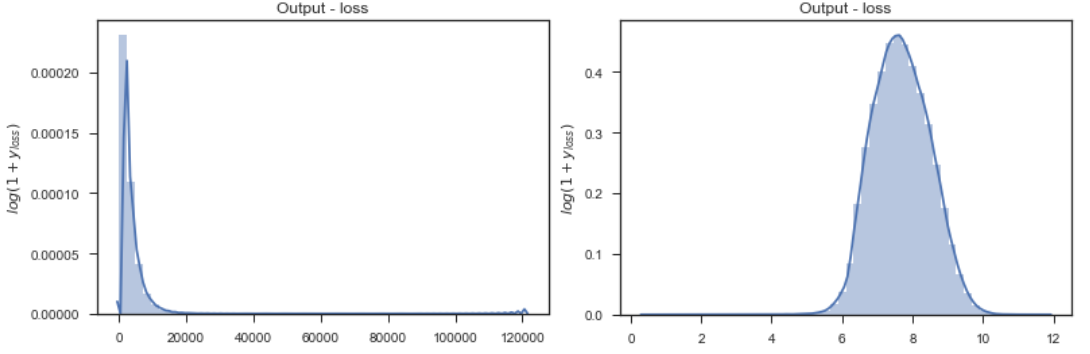
\includegraphics[width=.9\paperwidth]{Images/distribution-loss.png}}
\caption{Distribution plot of the output to the left and $log(1 + y_{loss})$ distribution to the right}
\label{fig:loss}
\end{figure}
\begin{figure}[H]
\centering
\makebox[\textwidth]{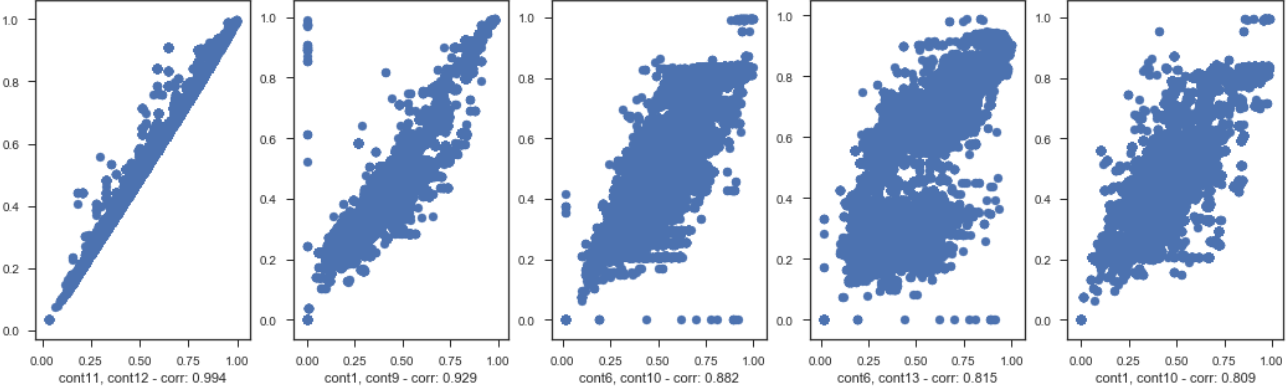
\includegraphics[width=.9\paperwidth]{Images/continuous-correlation.png}}
\caption{Five highest correlation pairs among continuous attributes}
\label{fig:con-corr}
\end{figure}
To start of the modeling process few test runs where executed with all of the models to get a feel of there potential. Since the output is highly skewed it was transformed with $y=log(1 + y)$ in order to correct for the skewness, assumed that the liner-models would then perform better. However the results obtained with log-transform where so far off that when executing the inverse with $x^y - 1$ resulted in overflow errors and thus making the experiments useless.
The highly correlated pairs of attributes where tackled by removing one from each pair, thus removing ['cont9', 'cont12', 'cat2', 'cat3', 'cat4', 'cat5', 'cat6', 'cat7', 'cat8', cat86].
\begin{table}[H]
\begin{tabular}{ |c|c|c|c| } 
\hline
Model & Training Error & Test Error & Parameters \\
\hline
LinearRegression & 1281.476 & 1655603234.882 & \\
Ridge & 1183.76 & 1302.587 & alpha=1.0 \\
Lasso & 1181.697 & 1305.573 & alpha=0.001 \\
ElasticNet & 1488.597 & 1512.204 & \\
KNeighborsRegressor & 1732.174 & 1747.104 & n\_neighbors=1 \\
SVR & 1753.704 & 1755.613 & \\
BaggingRegressor & 522.287 & 1295.292 & \\
RandomForestRegressor & 473.832 & 1245.477 & n\_estimators=50 \\
ExtraTreesRegressor & 0.0 & 1281.961 & n\_estimators=100 \\
GradientBoostingRegressor & 1223.819 & 1296.367 & loss='huber' \\
MLP (Scikit-Learn) & & 1229.617 & hidden\_layer\_sizes=(150,)\\
\hline
\end{tabular}
\caption{\label{tab:start}The first tests (*If not specified then the default Scikit-Learn parameters where used)}
\end{table}
The first test results are listed in \ref{tab:start}. The MLP and the tree models give promising results, since they give the lowest test error even though they seem to have overfitted the training data. \\\\
For the tree models a decision was made to study Gradient Boosting throughly since Scikit-Learn provides the Huber loss function \ref{eq:6} which is similar to MAE.
\begin{equation} \label{eq:6}
HuberLoss(y, \hat{y}) = \begin{cases} 
                  \frac{1}{2}(y - \hat{y})^2 & for\ |x|\leq \alpha \\
                  \alpha|y - \hat{y}|-\frac{1}{2}\alpha^2 & otherwise
               \end{cases}
\end{equation}
The Gradient Boosting has quite many parameters, in order to find the best combination of hyper-parameters a thorough grid scan was executed. The grid scan was executed for n\_estimators=[5, 50, 250, 500], alpha=[0.9, 0.5, 0.1], learning\_rate=[0.1, 0.0001], min\_samples\_leaf=[10, 20], min\_samples\_split=[10, 20] and max\_depth=[2, 3, 6]. The lowest mean absolute error of 1149.09 was obtained with (alpha=0.5, n\_estimators=250, max\_depth=6, learning\_rate=0.1, min\_samples\_leaf=20, min\_samples\_split=20), the result can be seen in figure~\ref{fig:gbr}.

\begin{figure}[H]
\centering
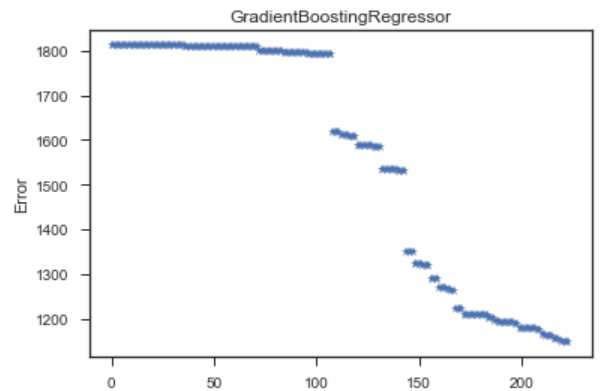
\includegraphics{Images/gbr.png}
\caption{Results for Gradient Boosting grid search}
\label{fig:gbr}
\end{figure}

\todo{Add more + MLP}

% * Fyrir verkefni #1 og #2: Töflur/myndir sem sýna t.d.
%   * Tíðnirit (e. histograms) fyrir stakar inntaksbreytur/úttaksbreytu, myndir sem sýna fylgni 2ja inntaksbreyta ofl.
%   * Nákvæmni einstakra líkana.
%   * Áhrif “hyperparametra” á gæði líkana.
%   * Yfirlit yfir inntaksbreytur sem mestu máli skipta.

% * Skrifið stutta lýsingu á því sem myndir og töflur sýna. Númerið allar myndir og töflur og notið númer þegar vísað er í úr texta (“Á mynd 2 má sjá …”) Gætið þess texti á myndum sé læsilegur (ekki of lítill).

% * Lýsið stuttlega tilraunum sem skiluðu litlu (“misheppnuðust”)

\section{Conclusion}
\todo{...}

% * Helstu ályktanir.
% * Næstu skref. (Hvernig mynduð þið halda áfram með verkefnið?)

\appendix
\setlength{\voffset}{0cm}
\setlength{\hoffset}{0cm}

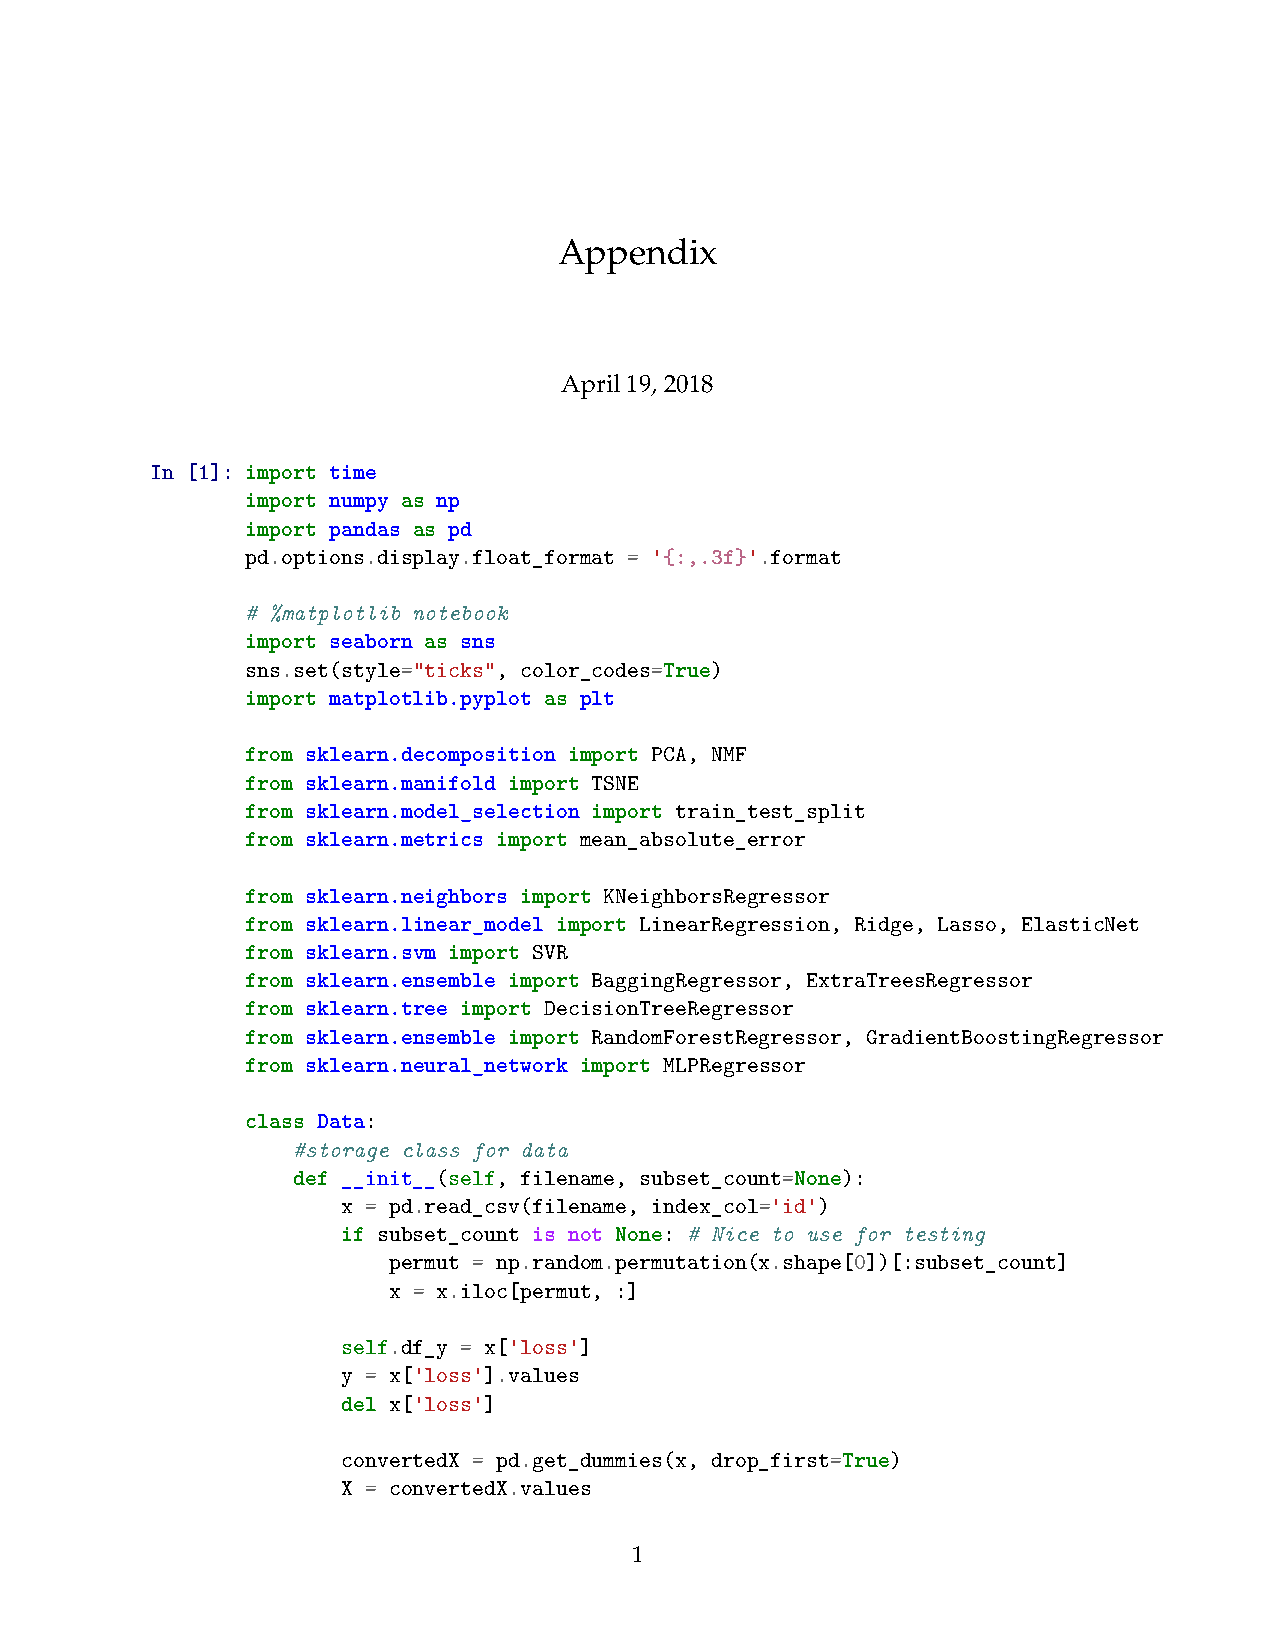
\includepdf[pages=-]{Images/Appendix.pdf}

\setlength{\voffset}{-2.54cm}
\setlength{\hoffset}{-2.54cm}

% For example, you can cite the Nano 3 Lecture notes \cite{nano3}.
% \newpage
% \begin{thebibliography}{9}
% \bibitem{nano3}
%   K. Grove-Rasmussen og Jesper Nygård,
%   \emph{Kvantefænomener i Nanosystemer}.
%   Niels Bohr Institute \& Nano-Science Center, Københavns Universitet
% \end{thebibliography}
\end{document}